\documentclass[tikz]{standalone}

\usepackage{pgfplots}
\usetikzlibrary{patterns}

\begin{document}
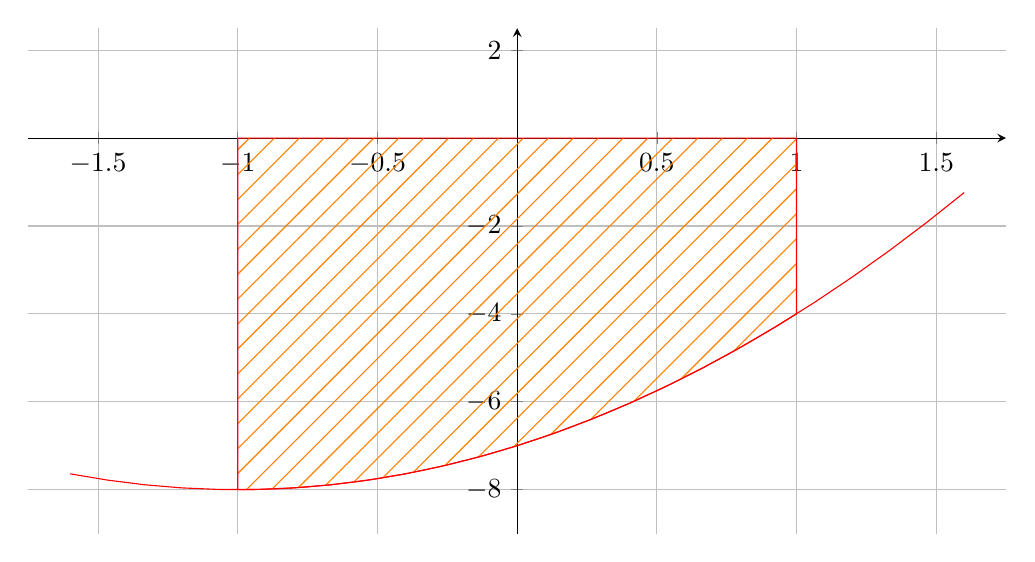
\begin{tikzpicture}
% diagonal fill pattern
\pgfdeclarepatternformonly{north east lines wide}%
   {\pgfqpoint{-1pt}{-1pt}}%
   {\pgfqpoint{10pt}{10pt}}%
   {\pgfqpoint{9pt}{9pt}}%
   {
        \pgfsetlinewidth{0.4pt}
        \pgfpathmoveto{\pgfqpoint{0pt}{0pt}}
        \pgfpathlineto{\pgfqpoint{9.1pt}{9.1pt}}
        \pgfusepath{stroke}
    }

    \begin{axis}[
        grid=major,
        axis lines=middle,
        xmin=-1.75,
        xmax=1.75,
        ymin=-9,
        ymax=2.5,
        width = 14cm,
        height = 8cm
    ]
    \addplot[color=red, domain=-1.6:1.6] {x^2 + 2*x - 7};
    %\addlegendentry{$x^2 + 2x - 7$}
    \addplot+[
        mark=none,
        domain=-1:1,
        pattern=north east lines wide,
        pattern color=red!50!yellow
        ] {x^2 + 2*x - 7} \closedcycle;
    \end{axis}
\end{tikzpicture}
\end{document}
